%***** Preamble *****%
\documentclass[a4paper]{article}

%% Language and font encodings
\usepackage[english]{babel}
\usepackage[utf8x]{inputenc}
\usepackage[T1]{fontenc}
\usepackage{graphicx}
\usepackage[font=small,labelfont=bf]{caption}
\usepackage{environ}
\usepackage{amsmath}

%% Sets page size and margins
\usepackage[a4paper,top=3cm,bottom=2cm,left=3cm,right=3cm,marginparwidth=1.75cm]{geometry}

%% Useful packages
\usepackage{amsmath}
\usepackage{graphicx}
\usepackage[colorinlistoftodos]{todonotes}
\usepackage[colorlinks=true, allcolors=blue]{hyperref}

\usepackage{float}  % Usado para posicionar imagens
\usepackage{enumitem} % Usado para criar listas enumeradas com letras
\usepackage{subcaption} % Usado para criar múltiplas imagens, uma ao lado da outra

\usepackage{tikz} % Usado para criar FSMs
\usetikzlibrary{automata, positioning, arrows}



\usepackage{listings}
\usepackage{color}
\usepackage{xcolor}

\definecolor{vgreen}{RGB}{104,180,104}
\definecolor{vblue}{RGB}{49,49,255}
\definecolor{vorange}{RGB}{255,143,102}

\lstdefinestyle{verilog-style}
{
    language=Verilog,
    basicstyle=\small\ttfamily,
    keywordstyle=\color{vblue},
    identifierstyle=\color{black},
    commentstyle=\color{vgreen},
    numbers=left,
    numberstyle=\tiny\color{black},
    numbersep=10pt,
    tabsize=4,
    moredelim=*[s][\colorIndex]{[}{]},
    literate=*{:}{:}1
}

\makeatletter
\newcommand*\@lbracket{[}
\newcommand*\@rbracket{]}
\newcommand*\@colon{:}
\newcommand*\colorIndex{%
    \edef\@temp{\the\lst@token}%
    \ifx\@temp\@lbracket \color{black}%
    \else\ifx\@temp\@rbracket \color{black}%
    \else\ifx\@temp\@colon \color{black}%
    \else \color{vorange}%
    \fi\fi\fi
}
\makeatother

\usepackage{trace}


\title{Curso de Verilog - Dia 4}
\author{Caio Rodrigo, Jorge Reis, Manuel Adahil}
\date{} % No Date
%%%%%%%%%%%%%%%%%%%%%%%%%%%%%%%%%%%%%%%%%%%%%%%%%%%%%%%%%%%%%%%%%
%***** Document *****%
\begin{document}
\maketitle

%***** Prática 6 - Moore FSM *****%
\section*{Prática 6 - Moore FSM}
Imagine o seguinte cruzamento:

\begin{figure}[H]
	\centering
    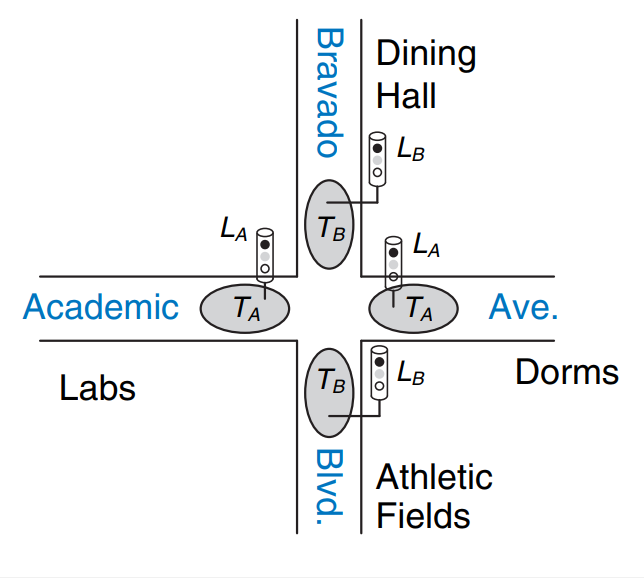
\includegraphics[width=0.4\textwidth]{images/cruzamento.PNG}
    \caption*{Cruzamento entre duas ruas.}
\end{figure}

Os elipses hachurados de cinza(TA e TB) são sensores que detectam se alguém está presente na área demarcada e os semáforos indicam se alguém pode passar ou não, possuindo três cores para o controle:

\begin{itemize}
		\item Vermelho - Pare;
		\item Amarelo - Atenção (Transição);
		\item Verde - Siga;
\end{itemize}

O controlador dos semáforos vai receber como entrada os dados do sensores TA e TB e  terá como saída a mudança das luzes, como visto na imagem:

\begin{figure}[H]
	\centering
    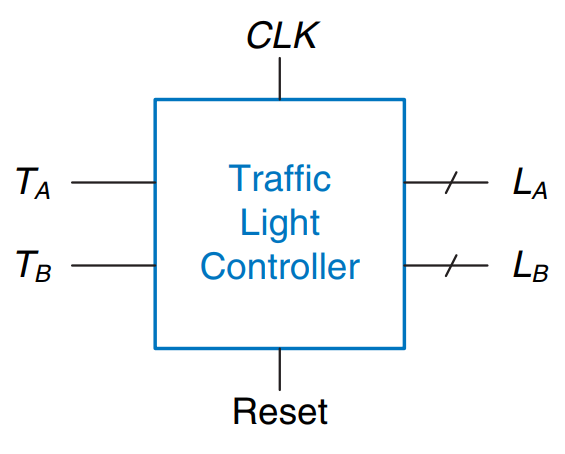
\includegraphics[width=0.4\textwidth]{images/controlador.PNG}
    \caption*{Controlador}
\end{figure}

O comportamento deste controlador é indicado pelas tabelas abaixo e pode ser modelado através de uma máquina de estados.

Faça a codificação e o testbench da máquina de estados de Moore que modela o sistema de tráfego explanado anteriormente. A máquina de estados é exibida a seguir:

\begin{figure}[H]
	\centering
    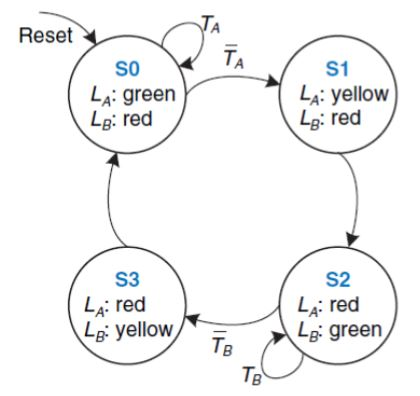
\includegraphics[width=0.4\textwidth]{images/Moore_FSM.jpg}
    \caption*{Moore FSM para o semáforo.}
\end{figure}

Lembre-se que uma FSM possui dois blocos de lógica combinacional, um para calcular o próximo estado (next state logic) e outro para definir a saída (output logic), e os registradores que armazenam o estado. Os registradores são atualizados em cada borda de subida do clock. 

Utilize as tabelas abaixo para codificar os estados, saídas e a transição de estados:

\begin{figure}[H]
\centering
\begin{subfigure}{.3\textwidth}
	\centering
    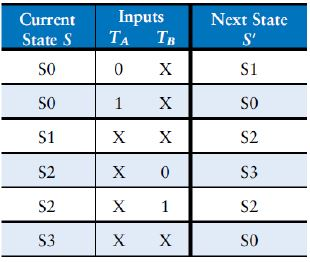
\includegraphics[width=.8\linewidth]{images/tabela_de_transicao_de_estados.jpg}
    \caption*{Tabela de transição de estados}
\end{subfigure}%
\begin{subfigure}{.3\textwidth}
	\centering
    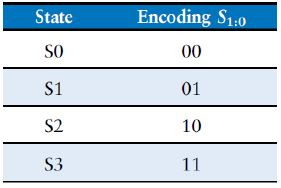
\includegraphics[width=.8\linewidth]{images/codificacao_de_estados.jpg}
    \caption*{Codificação dos estados}
\end{subfigure}%
\begin{subfigure}{.3\textwidth}
	\centering
    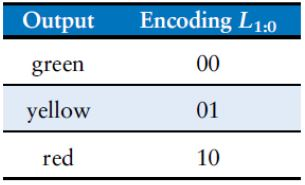
\includegraphics[width=.8\linewidth]{images/codificacao_de_saidas.jpg}
    \caption*{Codificação da saída}
\end{subfigure}
\end{figure}


%***** Prática 7 - Mealy FSM *****%

\section*{Prática 7 - Mealy FSM}

Modifique a FSM da questão anterior para uma FSM de Mealy. Faça a codificação e compare os testbenches das duas FSMs. \textbf{Dica}: você pode instanciar os dois módulos no testbench e testar os dois ao mesmo tempo para facilitar a comparação das ondas.

Em seguida, responda as seguintes questões:

\begin{enumerate}
\item O que foi modificado no código original (FSM de Moore) para codificar a FSM de Mealy?

\item Qual foi a mudança de comportamento em relação à saída da FSM de Moore? Ou seja, quando a saída é modificada na FSM de Moore e de Mealy?

\item A FSM de Mealy funciona corretamente?

\end{enumerate}

%%% NEWPAGE
\newpage
\section*{Fatality}
Implemente a FSM de Mealy abaixo bem como seu testbench. Repare que ela possui mais de uma entrada e saída para cada transição.

\begin{figure}[H]
	\centering
    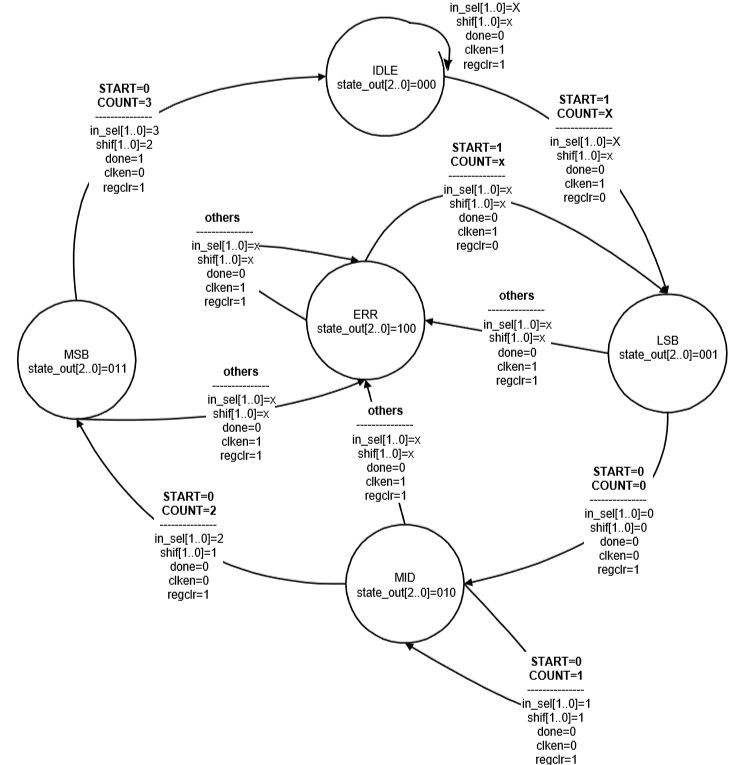
\includegraphics[width=.8\linewidth]{images/multicycle_multiplier.jpg}
    \caption*{FSM de Mealy de um multiplicador multicycle}
\end{figure}
\end{document}